% 2020 全国Ⅲ卷 理19：长方体 ABCD-A1B1C1D1，E 在 DD1、F 在 BB1 上
% 来源 PDF：普通高考/2020/2020全国3理(云南,广西,贵州,西藏,四川).pdf 第 2 页（A3 横排），印面 1126，第 19 题题干下方
% 结构（按原页矢量数据换算）：ABCD 为上底面，A1B1C1D1 为下底面；A 在前右、B 在后右、
%   C 在后左、D 在前左；AD = 1 为图面横向单位，AA1 = 3 为竖向单位，AB = 2 沿 45° 方向
%   以半长画出（原页即如此，AB 与 AD 在图面上等长）。
%   E 在棱 DD1 上且 2DE = ED1（自 D 向下三分之一处），F 在棱 BB1 上且 BF = 2FB1（自 B 向下三分之二处）。
% 实线：DA、AB、BC、CD、DD1、AA1、BB1、D1A1、A1B1 以及 AE、AF、A1E、A1F；
% 虚线：CC1（被遮挡的棱）、C1D1 与 C1B1（被遮挡的底棱）以及体内线段 EF。
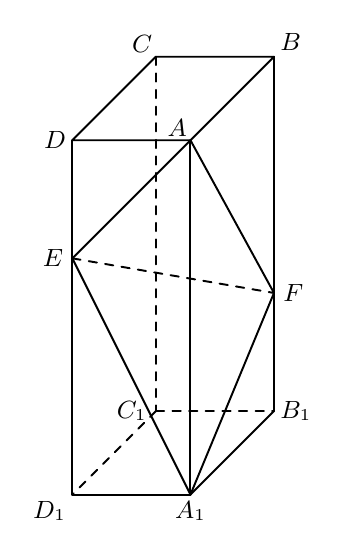
\begin{tikzpicture}[line width=0.7pt, font=\small,
  x=1.5cm, y=1.5cm, line cap=round, line join=round]

  % 顶点
  \coordinate (D)  at (0,3);
  \coordinate (A)  at (1,3);
  \coordinate (C)  at (0.70711,3.70711);
  \coordinate (B)  at (1.70711,3.70711);
  \coordinate (D1) at (0,0);
  \coordinate (A1) at (1,0);
  \coordinate (C1) at (0.70711,0.70711);
  \coordinate (B1) at (1.70711,0.70711);

  % E、F 按定比取点
  \coordinate (E) at (0,2);
  \coordinate (F) at (1.70711,1.70711);

  % 上底面
  \draw (D) -- (A) -- (B) -- (C) -- cycle;

  % 可见棱
  \draw (D) -- (D1);
  \draw (A) -- (A1);
  \draw (B) -- (B1);
  \draw (D1) -- (A1);
  \draw (A1) -- (B1);

  % 题设线段
  \draw (A) -- (E);
  \draw (A) -- (F);
  \draw (A1) -- (E);
  \draw (A1) -- (F);

  % 被遮挡的棱与体内线段
  \draw[dashed] (C) -- (C1);
  \draw[dashed] (C1) -- (D1);
  \draw[dashed] (C1) -- (B1);
  \draw[dashed] (E) -- (F);

  % 顶点标注
  \node[above left,  inner sep=1pt] at (C)  {$C$};
  \node[above right, inner sep=2pt] at (B)  {$B$};
  \node[left,        inner sep=2pt] at (D)  {$D$};
  \node[above left,  inner sep=1pt] at (A)  {$A$};
  \node[left,        inner sep=3pt] at (E)  {$E$};
  \node[right,       inner sep=3pt] at (F)  {$F$};
  \node[below left,  inner sep=2pt] at (D1) {$D_1$};
  \node[below,       inner sep=2pt] at (A1) {$A_1$};
  \node[left,        inner sep=3pt] at (C1) {$C_1$};
  \node[right,       inner sep=2pt] at (B1) {$B_1$};
\end{tikzpicture}
